\documentclass[../598comp.tex]{subfiles}

\graphicspath{ {./lectures/images/}{./images/} }

\date{05-19}

\begin{document}

\section{05-19}

Previously we were working with finite memory machines. Limitations on what we
could do even when we came to omega languages.

Two ways to recognize regular languages.
Regular languages in terms of deterministic finite automata, and regular expressions.

Now we are getting infinite memory. A finite state machine plus an auxiliary
stack. Then in the next module we will get two stacks.

\subsection{Context Free Languages}
We will define CFL's in terms of grammars.

We will define a grammar as a way to generate strings in the language. There is
a lot more structure than regex had. Rules for producing strings.

\begin{definition}[Context-free Grammar]
  A \ul{context-free grammar} consists of
  \begin{enumerate}
  \item 
    a set of symbols called terminals ($\Sigma$ alphabet)
  \item
    Another set of symbols called non-terminals or variables $V$.
  \item
    Both $V, \Sigma$ are finite, and $V \cap \Sigma = \varnothing$.
  \item
    A special variable called the start symbol, usually but not always $S$.
  \item
    A \ul{set} of rules called PRODUCTIONS.
    \begin{gather*}
      A \to \alpha, \ A \in V, \ \alpha \in (V \cup \Sigma)^*
    \end{gather*}
  \end{enumerate}
\end{definition}
\begin{example}
  Let $\Sigma = \{a, b\}$. These are our terminal symbols. Terminal suggests
  that something has to be terminated. Variable on the other hand suggests
  something that can change. $V = \{S\}$. Just the start symbol. Rules:
  \begin{gather*}
    S \to \epsilon, \ S \to aSb
  \end{gather*}
  Apply \ul{any rule} you like to replace a non-terminal with the RHS of a rule.
  It doesn't matter what the surrounding context is. This is why it's called
  context free.
  \begin{gather*}
    S \to aSb \to aaSbb \to aaaSbbb \to aaabbb
  \end{gather*}
  This allows you to create $\{a^nb^n \ | \ n \geq 0\}$, which is not a regular
  language. CFL's are clearly more powerful than regular languages.

  When you obtain a string with no more non-terminals, you have generated a
  string in the context free language.
  \begin{gather*}
    L(G) = \{w \in \Sigma^* \ | \ w \ \text{can be generated from the start
      symbol $S$}\}
  \end{gather*}
  Unlike with DFA the language is defined and then you have to recognize it,
  here you are generating the language.
\end{example}

\begin{example}[Grammar for arithmetic expressions]
  All modern programming languages, the syntax is a context free language,
  oftentimes it is even more restricted than that. Cobalt does not have a
  context free grammar, but now we've realized that this is a stupid idea. Every
  modern programming language is context free.
  \begin{gather*}
    \Sigma = \{0, 1, \cdots, 9, \times, +, (, )\} \\
    V = \{\langle EXP \rangle, \langle NUM \rangle, \langle NZ \rangle, \langle
    N \rangle\}
  \end{gather*}
  Start symbol $<EXP>$. Notation to save space.
  \begin{align*}
    \langle EXP \rangle &\to \langle EXP \rangle + \langle EXP \rangle \ | \
    \langle EXP \rangle \times \langle EXP \rangle \ | \ \langle EXP \rangle \ | \
    \langle NUM \rangle \\
    \langle NUM \rangle &\to 0 \ | \ \langle NZ \rangle \\
    \langle NZ \rangle &\to 1 \langle N \rangle \ | \ 2 \langle N \rangle \ | \
    \cdots \ | \ 9 \langle NZ \rangle \\
    \langle N \rangle &\to 0 \langle N \rangle \mid 1 \langle N \rangle \ | \ 2
    \langle N \rangle \ | \ \cdots \ | \ 9 \langle NZ \rangle \ | \ \epsilon
  \end{align*}
  NZ is to allow you to write zero but prevent you from writing 00. To properly
  display \ul{derivations}, we will use trees called parse trees.
  \\
  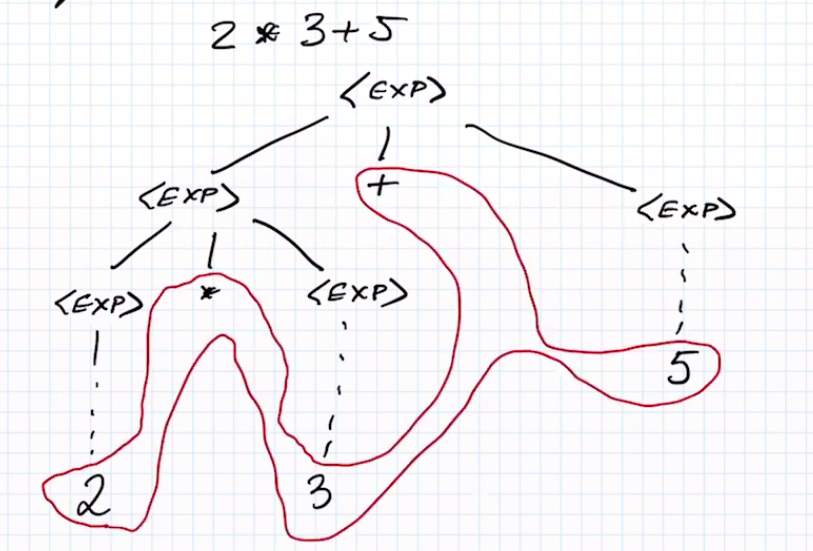
\includegraphics[width=\textwidth]{context_free_arithmetic_example.png}
\end{example}

\begin{definition}[Ambiguity in Context Free Languages]
  The grammar allows two (or more) distinct ways of parsing an expression. Such
  a grammar is called \ul{ambiguous}. An example of bad grammar engineering. A given
  language does not have a unique grammar. With regular languages there was a
  unique minimal automaton; there is no such concept in context free languages.

  It is possible to redesign the grammar so that it is \ul{not} ambiguous, at
  least in this case. There exist languages for which \ul{no} unambiguous
  language is possible. Then it is \ul{inherently ambiguous}.
\end{definition}

\subsection{Designing CFG}

\begin{example}[Counting CFG]
  How to produce the language $L = \{a^nb^{2n} \mid n \geq 0\}$. Rules:
  \begin{gather*}
    S \to aSbb \mid \epsilon
  \end{gather*}
  Keep going until you are happy and then wipe out the $S$.
  Notice that context free languages can count
\end{example}
\begin{example}[Palindromes]
  $L = \{x \in \Sigma^* \mid x = x^{REV}\}$. Rules:
  \begin{gather*}
    S \to aSa \mid bSb \mid a \mid b \mid \epsilon
  \end{gather*}
\end{example}
\begin{example}
  $L = \{x \in \Sigma^* \mid \#_a(x) = \#_b(x)\}$. A bit harder than example
  number 1. To make it easier let $d(x) = \#_b(x) - \#_a(x)$ and $L = \{x
  \mid d(x) = 0\}$.
  
  Let $x \in L$, and $u$ be the shortest prefix of $x$ such that $d(u) = 0$ and
  suppose $u$ starts with $b$. $u$ must end with $a$ because it starts with $b$.
  So $u = bva$ and $d(v) = 0$.
  
  $x = uz \Rightarrow d(z) = 0$
  \begin{gather*}
    S \to \epsilon \mid b SaS \mid aSbS \\
    \text{alternatively} \\
    S \to aSb \mid bSa \mid SS \mid \epsilon
  \end{gather*}
\end{example}

\begin{fact}
  Every regular language is a CFG.
\end{fact}

\begin{definition}
  A CFG is said to be in Chomsky Normal Form if every rule has the form
  \begin{gather*}
    A \to BC \ \text{or} \ A \to a
  \end{gather*}
  Here $A, B, C$ are non-terminals and $a$ is a terminal. We do not allow rules
  like $A \to \epsilon$ except for the start symbol. Some resources say that
  even the start symbol can't go to epsilon.
\end{definition}

\begin{theorem}
  Every context free language is generated by a context free grammar in chomsky
  normal form.
  \begin{proof}
    The idea is to systematically get rid of bad rules. e.g. $A \to \epsilon$ is
    a forbidden rule so throw it out and look at any rule with $A$ on the RHS
    e.g. $B \to \alpha_1A\alpha_2A$. Add all possible rules with some of these
    $A$'s removed. So in this case add the following rules.
    \begin{gather*}
      B \to \alpha_1\alpha_2A \\
      B \to \alpha_1A\alpha_2 \\
      B \to \alpha_1\alpha_2
    \end{gather*}
    Many other modifications of this type. Consider
    \begin{align*}
      &A \to x_1x_2x_3\cdots x_n, \ x_i \in \Sigma \cup V \\
      &\text{becomes} \\
      &A \to x_1A_1, x_1 \to x_1 \ \text{if} \ x_1 \in \Sigma \\
      &A_1 \to x_2 A_2, \ ...
    \end{align*}
    All these $A_i$ are new non terminals.
  \end{proof}
  You can see that there are lots of ways to modify the grammar while preserving
  the languages.
\end{theorem}

\subsection{Closure Properties of CFL's}
\begin{enumerate}
\item 
  $L_1, L_2$ are CFL's then $L_1 \cup L_2$ is a CFL.
  
  Let $S_1$ be the start for $G_1$ and $L(G_1) = L_1$, and $S_2$ be the start
  for $G_2$ and $L(G_2) = L_2$. Take all the rules together and add $S \to S_1
  \mid S_2$.
\item
  $L_1 \cdots L_2$ is also a context free language.
  \begin{gather*}
     \to S_1 S_2
  \end{gather*}
\item
  $L^*$ is a context free language if $L$ is. Add a new start symbol $S'$ and
  add the rule
  \begin{gather*}
    S' \to SS' \mid \epsilon
  \end{gather*}
\item
  CFL's are \ul{not} closed under
  \begin{enumerate}
  \item 
    intersection
  \item
    complement
  \end{enumerate}
\end{enumerate}
Easy proofs becaues of the power of grammars rather than fiddling with automata.

\begin{example}
  $L_1 = \{a^nb^nc^m \mid n, m \geq 0\}$ is a CFL, and so is $L_2 = \{a^mb^nc^n \mid n, m
  \geq 0\}$. Then $L_1 \cap L_2 = \{a^nb^nc^n \mid n \geq 0\}$. The idea is that
  when there is a buffer, you can't count. This is our favorite example of
  something that is not context free.
  
  Tomorrow we will see a new pumping lemma for context free languages.
  
  Note also that $L = \{a^nb^nc^n \mid n \geq 0\}$ is not a CFL but $\ol{L}$ is
  a CFL! Also see that if it were closed under complementation and under union
  it would have been closed under intersection. So it cannot possibly be closed
  under complementation.
\end{example}

\begin{proposition}
  If $L$ is a CFL and $R$ is a regular language then $L \cup R$ is a CFL.
\end{proposition}

\begin{fact}
  There is an algorithm to look at a grammar and decide if $L(G) = \varnothing$.
  It's easy to write grammars that don't produce anything. For example if you
  don't give a rule for the start symbol. No matter how many other rules you
  have it won't produce anything. It might be that you never get rid of the
  non-terminals, which by definition are not in the language. The point is that
  there is an algorithm that can look and decide.
  \begin{proof}
    DIY
  \end{proof}
\end{fact}

Algorithm to decide if $w \in L(G)$. Works on general context free grammar (even
ambiguous ones). To reduce the amount of book keeping assume $G$ is in chomsky normal form.

Typical dynamic programming algorithm. Given $G = (V, \Sigma, S, P)$. P for
the set of rules because they are referred to as productions. Input $w = a_1
\cdots a_n \in \Sigma^*, a_i \in \Sigma$. 

The idea is to work bottom up to construct a possible derivation for $w$. To get
a specific letter $a$ we must have used a rule of the form $A \to a$.

We define inductively a 2-indexed family of subsets of $V$. 
\begin{gather*}
  i \leq j, \ X_{ij} \coloneqq \{A \in V \mid A \to a_i \cdots a_j\} \\
  X_{ii} = \{A \in V \mid A \to a_i \}
\end{gather*}
When we come to compute $X_{ij}$, we assume that we have already computed
$X_{ij}, X_{kj}$ for all $k$ between $i$ and $j$
When we come to compute $X_{ij}$, we assume that we have already computed
$X_{ik}, X_{kj}$ for all $k$ between $i$ and $j$. So if $B \in X_{ik}$, $C \in
X_{(k + 1)j}$ and $A \to BC$ is a rule in $G$ then we put $A \in X_{ij}$.

\subsection{Algorithms For CFLs}
\begin{enumerate}
\item 
  $L(G) = \varnothing$ is decidable.
\item
  $L(G) \ \text{infinite}$  is decidable.
\item
  $L(G) = \Sigma^*$ is undecidable. This is surprising at first. Provably impossible.
\end{enumerate}

Start of a topic called parsing. Heavily studied in a compiler class. Reached
such a high state of understanding that nobody really needs to write parsers
anymore because people have written parser generators.

\subsection{Pushdown Automata}

This is an NFA + Stack (1 stack only, no more). Emphasis on NFA. Nondetermism is
built in to the structure. DFA pushdown automata are not equivalent to NFA
pushdown automata. There is an equivalent deterministic context free language.

\begin{theorem}
  Every CFL can be recognized by a PDA (pushdown automata) and every language
  recognized by a PDA is a CFL. A language is context free if and only if it is
  recognized by a PDA.
  
  Use judgement. Sometimes it is much easier to do a proof via PDA, and
  sometimes easier via grammar.
\end{theorem}

\begin{definition}[Pushdown Automata]
  $Q$ represents the states (finite).

  $\Sigma$ represents the input alphabet (finite). $\Sigma_\epsilon = \Sigma
  \cup \{\epsilon\}$.

  $\gamma$ represents the stack alphabet $\gamma \supset \Sigma, \
  \gamma_\epsilon = \gamma \cup \{\epsilon\}$

  $\delta: Q \times \Sigma_\epsilon \times \gamma_\epsilon \to P_f(Q \times \gamma_\epsilon)$ 

  $P_f$ is the finite power set.

  Reading a letter involves (i) looking at the input and the top of the stack,
  (ii) changing the state, (iii) poping the stack or pushing something on the
  stack or both and then move to the next input symbol.

  Notation, $a, b \to c$. $b$ is seen on top of the stack, $a$ is the next input
  symbol, pop the stack and replace $b$ with $c$. $a$ may be $\epsilon$ which
  would mean don't read input
  
  Reading a letter involves (i) looking at the input and the top of the stack,
  (ii) changing the state, (iii) poping the stack or pushing something on the
  stack or both and then move to the next input symbol.
  
  Notation, $a, b \to c$. $b$ is seen on top of the stack, $a$ is the next input
  symbol, pop the stack and replace $b$ with $c$.
  
  $a$ may be $\epsilon$ which would mean don't read input. $b$ may be $\epsilon$
  which would mean just push $c$. $c$ may be $\epsilon$ which would mean just pop
  the stack.
\end{definition}

\begin{example}
  \includegraphics[width=\textwidth]{pda_example}
  \\
  You are required to go all the way to the end of the input or you are jammed
  and rejected. This is an example of a deterministic machine but in general you
  can have non determinism.
\end{example}

\begin{example}
  $L = \{a^ib^jc^k \mid i, j, k \geq 0 \wedge (i = j \vee i = k)\}$
  \\
  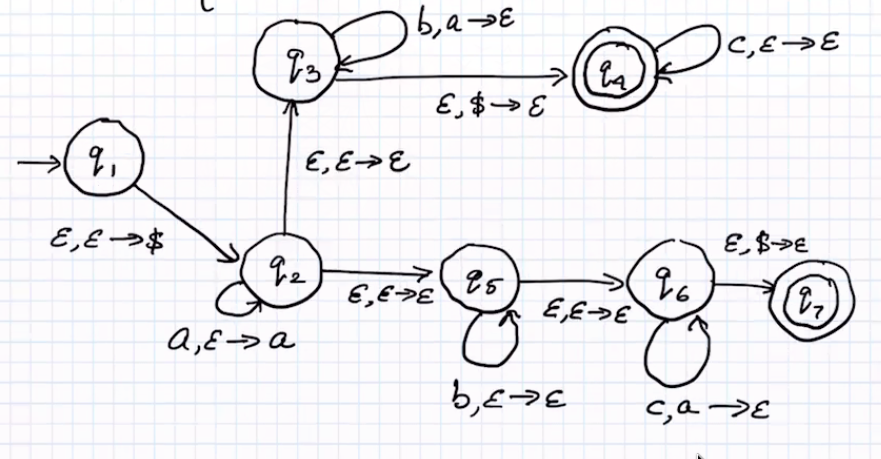
\includegraphics[width=\textwidth]{pda_example2}
  \begin{note}
    \begin{enumerate}
    \item[]
    \item 
      Acceptance only happens at the end
    \item
      A PDA cannot ``decide to jam'' when there are valid moves.
    \end{enumerate}
  \end{note}
\end{example}

\begin{note}
  There is an alternative notion of acceptance: no accept states, we accept if
  the stack is empty at the end of the input. These are equivalent.
\end{note}
$a^nb^nc^n$ cannot be accepted by a PDA because we can the a's and count off the
b's but then we don't know what to do with the c's. If we had \ul{2 stacks}, we
could accept $\{a^nb^nc^n \mid n \geq 0\}$ by pushing to the second stack as we
pop from the first stack.

$\{a^nb^nc^nd^n \mid n \geq 0\}$ still only needs 2 stacks, because you can go
back and forth between the two stacks. 2 stacks is enough for any number.
\begin{fact}
  A PDA with two stacks is \ul{universal}. i.e. it has the same power as a
  turing machine and can compute any computable function.

  People realized that complexity is more significiant than power, because the
  power of everything is the same once you get to two stacks, two queues, etc.
\end{fact}

\end{document}